\begin{figure}[htbp]
\centering
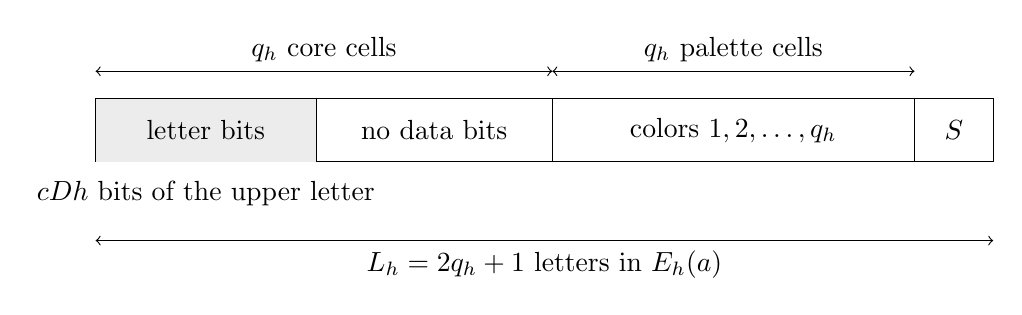
\begin{tikzpicture}[x=1cm,y=1cm]
 \draw (0,0) rectangle (11.4,0.8);
 \fill[gray!15] (0,0) rectangle (2.8,0.8);
 \draw (2.8,0)--(2.8,0.8);
 \draw (5.8,0)--(5.8,0.8);
 \draw (10.4,0)--(10.4,0.8);
 \node at (1.4,0.4) {letter bits};
 \node at (4.3,0.4) {no data bits};
 \node at (8.1,0.4) {colors $1,2,\ldots,q_h$};
 \node at (10.9,0.4) {$S$};
 \draw[<->] (0,1.15)--(5.8,1.15);
 \node[above] at (2.9,1.15) {$q_h$ core cells};
 \draw[<->] (5.8,1.15)--(10.4,1.15);
 \node[above] at (8.1,1.15) {$q_h$ palette cells};
 \node[below,align=center] at (1.4,-0.12) {$cDh$ bits of the upper letter};
 \draw[<->] (0,-1.0)--(11.4,-1.0);
 \node[below] at (5.7,-1.0) {$L_h=2q_h+1$ letters in $E_h(a)$};
\end{tikzpicture}
\caption{A canonical block encoding one letter $a\in\Sigma_{Dh}$.
The core carries its $cDh$ data bits, the palette contains each color
once in increasing order, and the stop cell closes the block. Both
control tracks are idle. The widths are schematic; the data positions
fit inside the core by the choice of $h_0$.}
\label{fr:block-figure}
\end{figure}
